\documentclass[11pt]{article}
\usepackage{fullpage}
\usepackage{graphicx}
\usepackage{amsmath}
\usepackage{amssymb}
\usepackage{verbatim}
\usepackage{xspace}
\usepackage{tikz}

\begin{document}

\title{Notes on Variational Inference}

\author{}

\maketitle

\section{Intro}
Suppose we have
\begin{align*}
\mu &\sim \mathcal{N}(u_0, (\lambda_0 \tau)^{-1}) \\
\tau &\sim \text{Gamma}(a_0, b_0) \\
x_i &\sim \mathcal{N}(\mu, \tau^{-1}) \; \text{for} \; i \in 1 \dots N
\end{align*}

with hyperparameters $a_0$, $b_0$, $\mu_0$, and $\lambda_0$,
and we want to find a distribution $q(\mu, \tau)$ over parameters $\mu$ and $\tau$
that best approximates the posterior $p(\mu, \tau | X)$ given the data $X = x_{1\dots N}$.

This corresponds to the directed graphical model below.

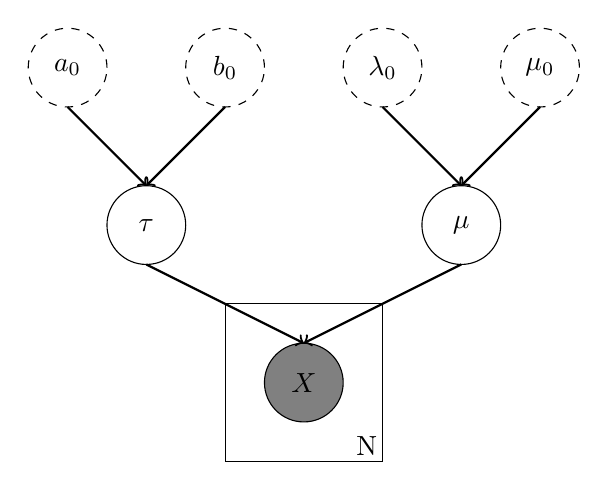
\begin{tikzpicture}
\draw[dashed] (0, 4) circle (0.5cm) node {$a_0$};
\draw[dashed] (2, 4) circle (0.5cm) node {$b_0$};
\draw[dashed] (4, 4) circle (0.5cm) node {$\lambda_0$};
\draw[dashed] (6, 4) circle (0.5cm) node {$\mu_0$};
\draw (1, 2) circle (0.5cm) node {$\tau$};
\draw (5, 2) circle (0.5cm) node {$\mu$};
\filldraw[fill=gray] (3, 0) circle (0.5cm) node {$X$};
\draw[thick,->] (0, 3.5) -- (1, 2.5);
\draw[thick,->] (2, 3.5) -- (1, 2.5);
\draw[thick,->] (4, 3.5) -- (5, 2.5);
\draw[thick,->] (6, 3.5) -- (5, 2.5);
\draw[thick,->] (1, 1.5) -- (3, 0.5);
\draw[thick,->] (5, 1.5) -- (3, 0.5);
\draw (2, -1) -- (2, 1);
\draw (2, 1) -- (4, 1);
\draw (4, 1) -- (4, -1);
\draw (4, -1) -- (2, -1);
\node[draw=none] at (3.8,-0.8) {N};
\end{tikzpicture}

We can write $p(X, \mu, \tau) = p(\tau | a_0, b_0) \cdot p(\mu | \tau, \mu_0, \lambda_0) \cdot \prod_{i=1}^N p(x_i | \mu, \tau)$.

Furthermore we know that
\begin{align*}
p(\tau|a_0, b_0) &= \frac{1}{\Gamma(a_0)} b_0^{a_0} \tau^{a_0 - 1} e^{-b_0\tau} \\
p(\mu | \tau, \mu_0, \lambda_0) &= \sqrt{\frac{\lambda_0 \tau}{2\pi}} e^{-(\frac{1}{2}\mu - \mu_0)^2\lambda_0\tau} \\
p(x_i | \mu, \tau) &= \sqrt{\frac{\tau}{2\pi}}e^{-\frac{1}{2}(x_i - \mu)^2 \tau}
\end{align*}

This allows us to write
\begin{align*}
\ln p(X, \mu, \tau) &= \ln p(\tau | a_0, b_0) + \ln p(\mu | \tau, \mu_0, \lambda_0) + \sum_{i=1}^N \ln p(x_i | \mu, \tau) \\
&= \big[ -\ln \Gamma(a_0) + a_0 \ln b_0 + (a_0 - 1) \ln \tau - b_0 \tau \big] \\
&+ \big[ \frac{1}{2}\ln \lambda_0 + \frac{1}{2}\ln \tau - \frac{1}{2} \ln 2\pi - \frac{1}{2} (\mu - \mu_0)^2 \lambda_0 \tau \big] \\
&+ \sum_{i=1}^{N} \big[ \frac{1}{2}\ln \tau - \frac{1}{2} \ln 2\pi - \frac{1}{2} (x - \mu)^2 \tau \big] \\
&= \big[(a_0 - 1) \ln \tau - b_0 \tau \big] + \big[ \frac{1}{2} \ln \tau - \frac{1}{2}(\mu - \mu_0)^2 \lambda_0 \tau \big] + \sum_{i=1}^{N} \big[ \frac{1}{2} \ln \tau - \frac{1}{2} (x- \mu)^2 \tau \big] + C \\
&= \big[ (a_0 - 1) + \frac{1}{2} + \frac{N}{2} \big] \ln \tau - \big[ \frac{1}{2}(\mu - \mu_0)^2 \lambda_0 + \sum_{i=1}^N \frac{1}{2}(x_i - \mu)^2 + b_0 \big] \tau + C
\end{align*}

Now we will assume that $q(\mu, \tau)$ factors cleanly, such that $q(\mu, \tau) = q_\mu(\mu) q_\tau(\tau)$. This isn't actually true, but if it's approximately true we can use this assumption to get a good approximation algorithm.

So we now will write that $q_\mu(\mu) = \mathbb{E}_\tau \big[ p(X, \mu, \tau) \big]$ and $q_\tau(\tau) = \mathbb{E}_\mu \big[ p(X, \mu, \tau) \big]$.

\section{Derivation of $q_\mu$}
First we will seek to evaluate $q_\mu(\mu)$.
We have that 
\begin{align*}
\ln q_\mu(\mu) &= \mathbb{E}_\tau \Big[ \big[ (a_0 - 1) + \frac{1}{2} + \frac{N}{2} \big] \ln \tau - \big[ \frac{1}{2}(\mu - \mu_0)^2 \lambda_0 + \sum_{i=1}^N \frac{1}{2}(x_i - \mu)^2 + b_0 \big] \tau \Big] + C \\
&= \mathbb{E}_\tau \Big[ \big[ -\frac{1}{2}(\mu - \mu_0)^2 \lambda_0 - \sum_{i=1}^N \frac{1}{2}(x_i - \mu)^2 \big] \tau \Big] + C_2 \\
&= -\frac{\mathbb{E}_\tau [\tau]}{2} \big[ (\mu - \mu_0)^2 \lambda_0 + \sum_{i=1}^N (x_i - \mu)^2 \big] + C_2
\end{align*}

We now clearly see that $\ln q_\mu(\mu)$ is a quadratic in $\mu$, so $q_\mu(\mu)$ itself must be a Gaussian. Solving for the precise parameters of this Gaussian can be done by expanding, grouping like terms, and completing the square:

\begin{align*}
\ln q_\mu(\mu) &= -\frac{\mathbb{E}_\tau [\tau]}{2} \big[ (\mu - \mu_0)^2 \lambda_0 + \sum_{i=1}^N (x_i - \mu)^2 \big] + C_2 \\
&= -\frac{\mathbb{E}_\tau [\tau]}{2} \big[ (\mu^2 + \mu_0^2 - 2\mu\mu_0) \lambda_0 + \sum_{i=1}^N x_i^2 + \mu^2 - 2x_i\mu \big] + C_2 \\
&= -\frac{\mathbb{E}_\tau [\tau]}{2} \big[ \mu^2\lambda_0 + \mu_0^2\lambda_0 - 2\mu\mu_0\lambda_0 + \sum_{i=1}^N x_i^2 + N \mu^2 - 2\mu \sum_{i=1}^N x_i \big] + C_2 \\
&= -\frac{\mathbb{E}_\tau [\tau]}{2} \big[ (\lambda_0 + N)\mu^2 - 2(\mu_0\lambda_0 + \sum_{i=1}^N x_i)\mu + (\mu_0^2\lambda_0 + \sum_{i=1}^N x_i^2 ) \big] + C_2 \\
&= -\frac{\mathbb{E}_\tau [\tau]}{2} \big[ \sqrt{\lambda_0 + N}\mu - \frac{(\mu_0\lambda_0 + \sum_{i=1}^N x_i)}{\sqrt{\lambda_0 + N}} \big]^2 + C_3 \\
&= -\frac{\mathbb{E}_\tau [\tau](\lambda_0 + N)}{2} \big[ \mu - \frac{(\mu_0\lambda_0 + \sum_{i=1}^N x_i)}{\lambda_0 + N} \big]^2 + C_3 \\
\end{align*}

Now let us compare this to the form of the log of a normal distribution:
\begin{align*}
\mathcal{N}(x | \mu, \tau^{-1}) &= \sqrt{\frac{\tau}{2\pi}} e^{-\tau(x - \mu)^2} \\
\ln \mathcal{N}(x | \mu, \tau^{-1}) &= \frac{1}{2} \ln \tau - \frac{1}{2} (2\pi) - \tau(x - \mu)^2 \\
\ln \mathcal{N}(x | \mu, \tau^{-1}) &= -\frac{1}{2} \big( - \ln \tau + \ln 2 + \ln \pi + \tau(x - \mu)^2 \big) \\
\ln \mathcal{N}(x | \mu, \tau^{-1}) &= -\frac{\tau}{2} (x - \mu)^2 + C \\
\end{align*}

We can see that $q_\mu(\mu) = \mathcal{N} \Big(\mu | \frac{\mu_0\lambda_0 + \sum_{i=1}^{N} x_i}{\lambda_0 + N}, \big(\mathbb{E}_{\tau}[\tau](\lambda_0 + N) \big)^{-1} \Big)$.

\section{Derivation of $q_\tau$}
Now we will seek to do the same for $q_\tau(\tau)$.

\begin{align*}
q_\tau(\tau) &= \mathbb{E}_\mu \big[ p(X, \mu, \tau) \big] \\
&= \mathbb{E}_\mu \Big[ \big[ (a_0 - 1) + \frac{1}{2} + \frac{N}{2} \big] \ln \tau - \big[ \frac{1}{2}(\mu - \mu_0)^2 \lambda_0 + \sum_{i=1}^N \frac{1}{2}(x_i - \mu)^2 + b_0 \big] \tau \Big] + C \\
&= \big[ (a_0 - 1) + \frac{1}{2} + \frac{N}{2} \big] \ln \tau - \mathbb{E}_\mu \big[ \frac{1}{2}\lambda_0(\mu - \mu_0)^2 + \frac{1}{2}\sum_{i=1}^N(x_i - \mu)^2 + b_0\big] \tau + C \\
\end{align*}

We compare this to the form of the log of a gamma distribution:
\begin{align*}
\text{Gamma}(x | a, b) &= \frac{1}{\Gamma(a)} b^a x^{a-1} e^{-bx} \\
\ln \text{Gamma}(x | a, b) &= -\ln \Gamma(a) + a \ln b + (a - 1) \ln x - bx \\
&= (a - 1) \ln x - bx + C
\end{align*}

So we quickly see that $q_\tau(\tau) = \text{Gamma}(\tau | a_0 + \frac{1 + N}{2}, \mathbb{E}_\mu[\frac{1}{2}\lambda_0(\mu - \mu_0)^2 + \frac{1}{2}\sum_{i=1}^N (x_i - \mu)^2 + b_0 ])$

\section{Deriving the update rule}
Recall that the mean of $\mathcal{N}(x | \mu, \tau^{-1}) = \mu$ and the mean of $\text{Gamma}(x | a, b) = \frac{a}{b}$.
Also note that the mean of our $\mu$ does not in fact depend on $\tau$ at all!

Thus we can immediately establish the value $\mu^* = \frac{\mu_0\lambda_0 + \sum_{i=1}^{N} x_i}{\lambda_0 + N}$.
Furthermore we can let $a^* = a_0 + \frac{1 + N}{2}$ and we can write $b = \mathbb{E}_\mu[\frac{1}{2}\lambda_0(\mu - \mu_0)^2 + \frac{1}{2}\sum_{i=1}^N (x_i - \mu)^2 + b_0]$.
Let us expand this expression for $b$ a bit:

\begin{align*}
b &= \mathbb{E}_\mu[\frac{1}{2}\lambda_0(\mu - \mu_0)^2 + \frac{1}{2}\sum_{i=1}^N (x_i - \mu)^2 + b_0] \\
&= \mathbb{E}_\mu[ \frac{1}{2}\lambda_0\mu^2 - \lambda_0\mu\mu_0 + \frac{1}{2}\lambda_0\mu_0^2 + \frac{1}{2}\sum_{i=1}^N x_i^2 - \frac{1}{2}\sum_{i=1}^N 2x_i\mu + \frac{1}{2}\sum_{i=1}^N \mu^2 + b_0] \\
&= \frac{1}{2}\lambda_0\mathbb{E}_\mu[\mu^2] - \lambda_0\mu_0 \mathbb{E}_\mu[\mu] + \frac{1}{2}\lambda_0\mu_0^2 + \frac{1}{2}\sum_{i=1}^N x_i^2 - \mathbb{E}_\mu[\mu] \sum_{i=1}^N x_i + \frac{N}{2}\mathbb{E}_\mu[\mu^2] + b_0 \\
&= (\frac{1}{2}\lambda_0 + \frac{N}{2}) \mathbb{E}_\mu[\mu^2] - (\lambda_0\mu_0 + \sum_{i=1}^Nx_i) \mathbb{E}_\mu[\mu] + (\frac{1}{2}\lambda_0\mu_0^2 + \frac{1}{2}\sum_{i=1}^N x_i^2 + b_0)
\end{align*}

Now we can use the facts that $\text{Var}[X] = \mathbb{E}[X^2] - \mathbb{E}[X]^2$ and $\text{Var}[\mathcal{N}(\mu, \tau^{-1})] = \tau^{-1}$ to rewrite the last line:

\begin{align*}
b &= (\frac{1}{2}\lambda_0 + \frac{N}{2}) \mathbb{E}_\mu[\mu^2] - (\lambda_0\mu_0 + \sum_{i=1}^Nx_i) \mathbb{E}_\mu[\mu] + (\frac{1}{2}\lambda_0\mu_0^2 + \frac{1}{2}\sum_{i=1}^N x_i^2 + b_0) \\
&= (\frac{1}{2}\lambda_0 + \frac{N}{2}) (\text{Var}[\mu] + \mathbb{E}[\mu]^2) - (\lambda_0\mu_0 + \sum_{i=1}^Nx_i) \mathbb{E}_\mu[\mu] + (\frac{1}{2}\lambda_0\mu_0^2 + \frac{1}{2}\sum_{i=1}^N x_i^2 + b_0) \\
&= (\frac{1}{2}\lambda_0 + \frac{N}{2}) \Big(\big(\mathbb{E}_{\tau}[\tau](\lambda_0 + N) \big)^{-1} + \mu^2\Big) - (\lambda_0\mu_0 + \sum_{i=1}^Nx_i) \mu + (\frac{1}{2}\lambda_0\mu_0^2 + \frac{1}{2}\sum_{i=1}^N x_i^2 + b_0) \\
\end{align*}

We now have an expression for $b$ in terms of $\mathbb{E}[\tau]$.
Furthermore, we know that $\mathbb{E}[\tau] = \frac{a}{b} = \frac{a_0 + \frac{1 + N}{2}}{b}$,
so we also have an expression for $\mathbb{E}[\tau]$ in terms of $b$.
Thus we can naturally employ an EM-like algorithm, alternately re-computing $b$ and $\mathbb{E}[\tau]$ variable in turn, to achieve an accurate approximation.

\section{Open Questions}
\begin{itemize}
\item Why the heck is $\lambda_0$ necessary?
\end{itemize}
\end{document}
